\documentclass[../diplomski_rad.tex]{subfiles}

\begin{document}

\sloppy

\justifying

\section{Pregled metoda mjerenja bioimpedancije}

Mjerenje bioimpedancije (engl. \textit{Bioelectrical Impedance Analysis; BIA})  dijelimo na 
analizu jednom frekvencijom (engl. \textit{Single frequency BIA; SF-BIA}) 
i analizu na više frekvencija(engl. \textit{Multi frequency BIA; MF-BIA}). 
Važna metoda je i bioelektrička spektrografija (engl. \textit{Bioelectrical spectroscopy; BIS}) 
koja daje rezultate kroz širok raspon frekvencija. 

SF-BIA je najjednostavnija i najbrža metoda jer koristi samo mjerenje impedancije jednom frekvencijom, najčešće 50 kHz. 
Iz izmjerene bioimpedancije matematičkim izračunima dobivaju se ukupna tjelesna voda, mišićna masa i masa masnog tkiva. 
Ova metoda ima najmanju preciznost jer se podatci prikupljaju na samo jednoj frekvenciji uzbudne struje.

MF-BIA koristi nekoliko različitih frekvencija čime se postiže veća točnost i mogućnost procjene dodatnih parametara, 
kao što su količine intracelularne i ekstracelularne vode. To je moguće jer stanična membrana blokira struju na niskim frekvencijama, 
a propušta ju na višim. 

Bioelektrička spektrografija najpreciznija je metoda mjerenja bioimpedancije. 
Mjerenja se vrše na širokom rasponu frekvencija, od 1 kHz do 1 MHz.  
Ovom metodom možemo procijeniti otpor na nultoj i beskonačnoj frekvenciji, parametre iz Cole modela bioimpedancije 
opisane u prethodnom poglavlju. 
Mjerenje BIS metodom zbog mnogo frekvencija traje duže i matematički izračuni su kompliciraniji, 
ali pruža  detaljniju i precizniju analizu sastava ljudskog tijela

Postupak mjerenja bioimpedancije svih ranije opisanih metoda je puštanje slabe, 
frekvencijski ovisne izmjenične struje kroz tkivo te mjerenje pada napona. 
Zatim se impedancija izračunava prema:
\begin{equation}
    \label{jed:prvajednadzba}
    Z\angle\theta = \frac{U\angle\theta_{1}}{I\angle\theta_{2}} 
\end{equation} 

Pri mjerenju bioimpedancije razlikujemo dvožično i četverožično spajanje elektroda. 
Kod dvožičnog mjerenja isti par elektroda služi za pobudnu struju i za mjerenje napona. 
Zbog toga dolazi do greške u mjerenju napona uzrokovane padom napona na elektrodama. 
Četverožično mjerenje je preciznije jer se pad napona mjeri direktno na koži i zbog toga će se koristiti u ovom radu \cite{Abasi2022}. 

\begin{figure}[htb]
    \centering
    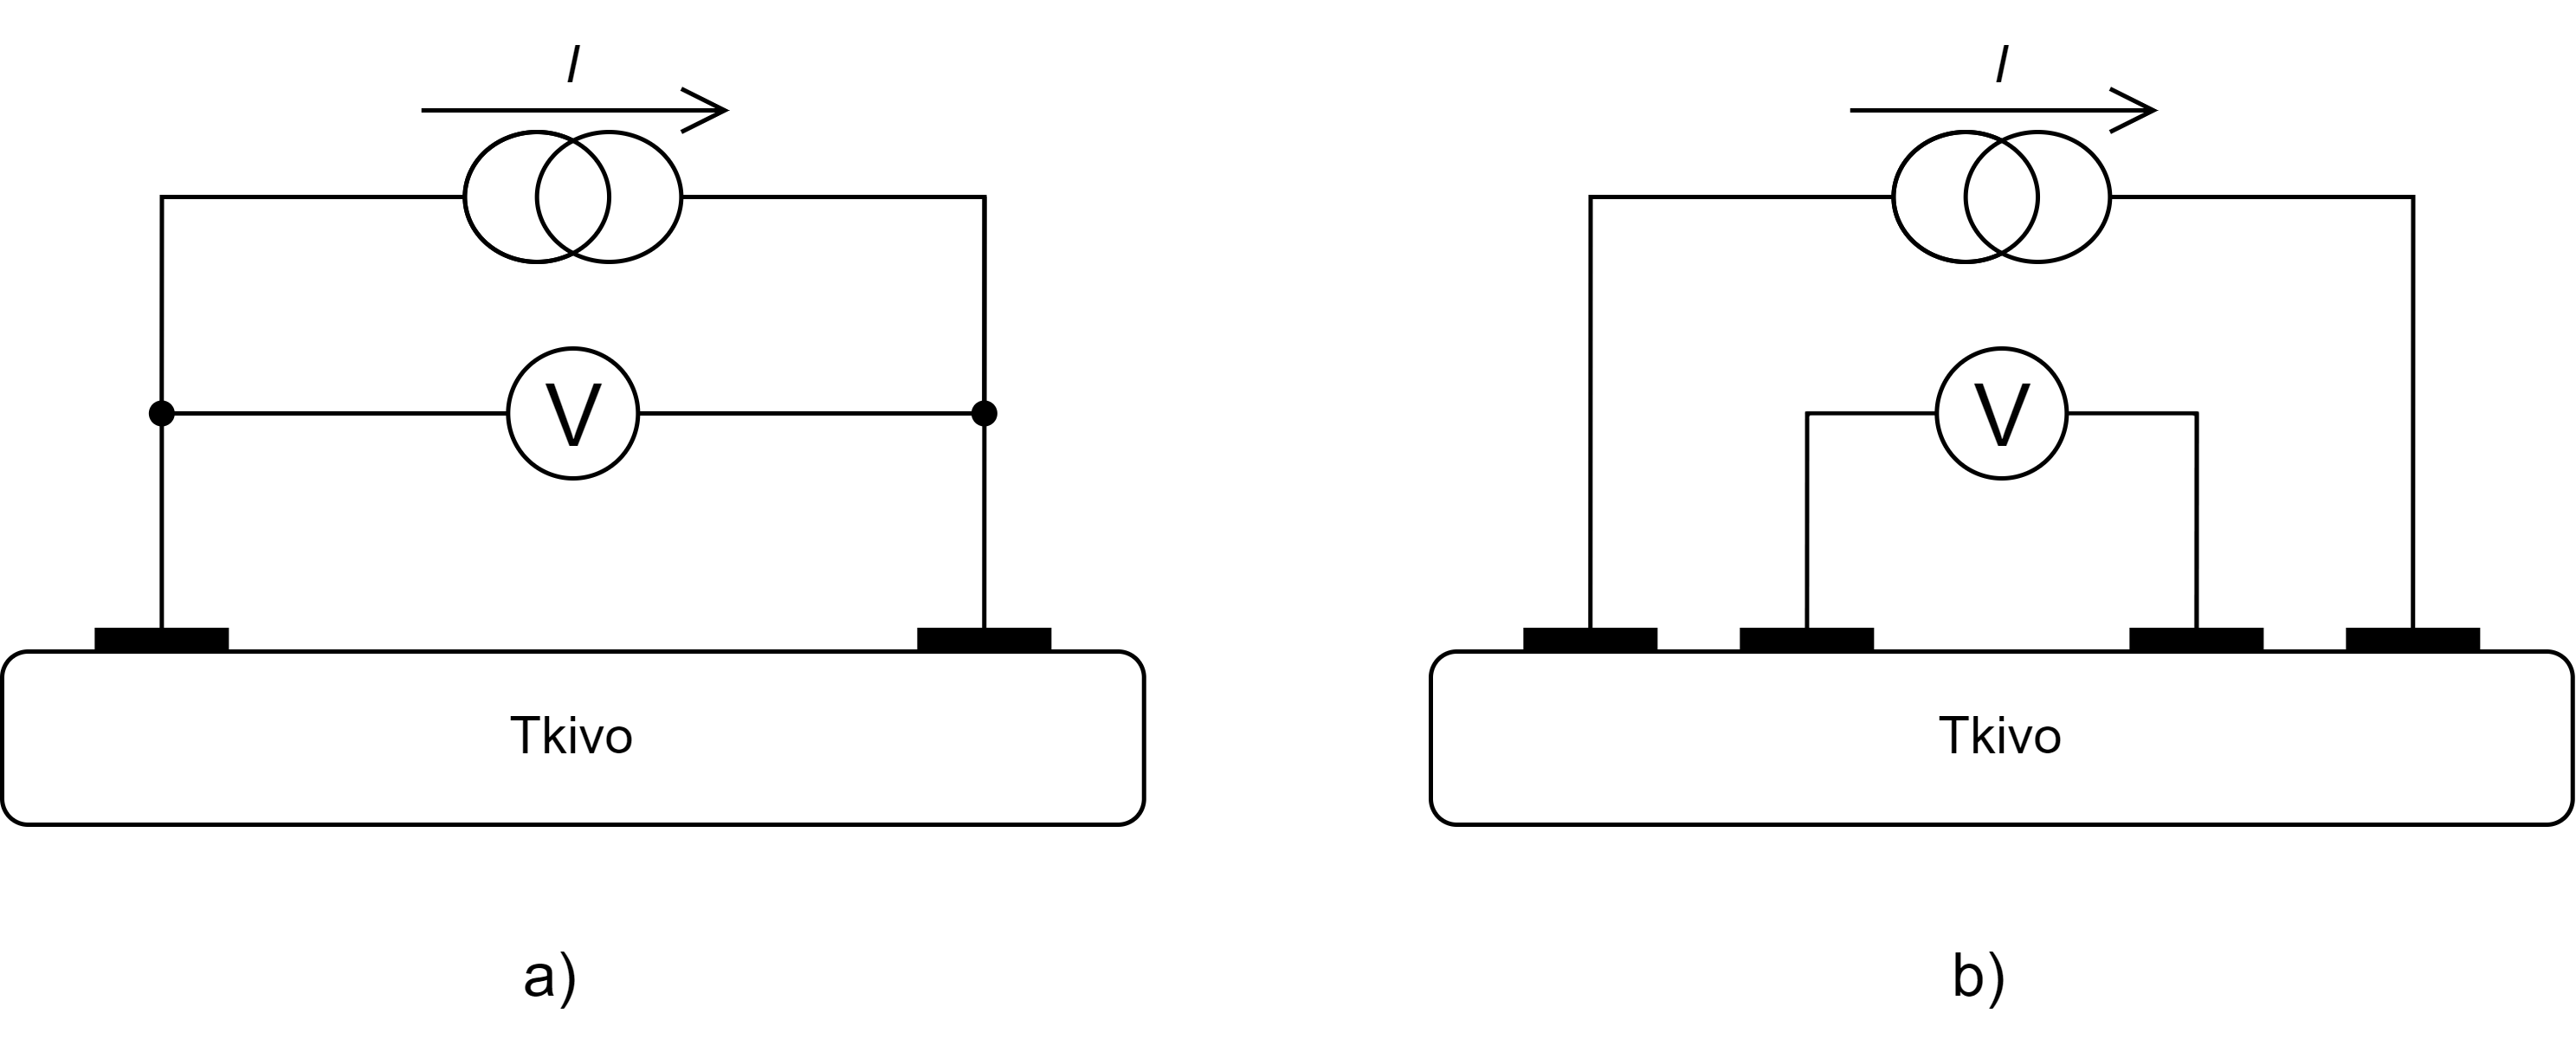
\includegraphics[width=0.8\textwidth]{Figures/dvo_vs_cetverozicno.png} 
    \caption{Dvožično (a) i četverožično (b) mjerenje bioimpedancije}
    \label{slk:cole_model}
\end{figure}

Važan dio mjernog sustava su i elektrode, koje kroz sučelje koža-elektroda omogućavaju protjecanje struje od mjernog sustava do tkiva. 
U ovom radu usporedit će se rezultati s dvama različitim vrstama elektroda, tradicionalnim metalnim elektrodama te tekstilnim elektrodama. 
Tekstilne elektrode izrađene su od tkanina impregniranih provodnim materijalima, najčešće srebrom. 
Njihova najveća prednost je udobnost i fleksibilnost te mogućnost integracije u odjeću.
Tako ih pacijenti neometano mogu nositi tijekom svakodnevnih aktivnosti i dužeg perioda. 
Međutim, metalne elektrode su manje osjetljive na vanjske parametre kao što su temperatura i znojenje kože što daje pouzdanije rezultate mjerenja. 
\cite{Meding2021}

\begin{figure}[htb]
    \centering
    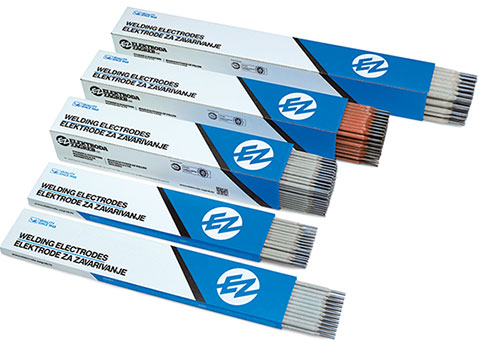
\includegraphics[width=0.6\textwidth]{Figures/electrode.jpg} 
    \caption{Tu će bit neka lijepa slika elektroda}
    \label{slk:elektrode}
\end{figure}

Sve opisane metode predstavljaju jednostavan i neinvazivan postupak mjerenja bioimpedancije. 
Važno je napomenuti kako izmjerena impedancija ovisi o brojim faktorima kao što su položaj tijela, hidracija, temperatura tijela i drugi 
što treba uzeti u obzir pri obradi rezultata mjerenja.

\section{Komercijalni uređaji za mjerenje bioimpedancije}

SFB7 ImpediMed

\end{document}